%
% File emnlp2018.tex
%
%% Based on the style files for EMNLP 2018, which were
%% Based on the style files for ACL 2018, which were
%% Based on the style files for ACL-2015, with some improvements
%%  taken from the NAACL-2016 style
%% Based on the style files for ACL-2014, which were, in turn,
%% based on ACL-2013, ACL-2012, ACL-2011, ACL-2010, ACL-IJCNLP-2009,
%% EACL-2009, IJCNLP-2008...
%% Based on the style files for EACL 2006 by 
%%e.agirre@ehu.es or Sergi.Balari@uab.es
%% and that of ACL 08 by Joakim Nivre and Noah Smith

\documentclass[11pt,a4paper]{article}
\usepackage[hyperref]{emnlp2018}
\usepackage{times}
\usepackage{url}
\usepackage{amsmath,amsfonts,amssymb}
\usepackage{paralist}
\usepackage{color,xcolor}
\usepackage{bm}
\usepackage{multirow}
\usepackage{makecell}
\usepackage{todonotes}

\newcommand{\rmx}{\mathrm x} % bold x for equations
\newcommand{\tabh}[1]{\multicolumn{1}{c|}{\textbf{#1}}}  % used for table headers
\newcommand{\tabc}[2]{\multicolumn{1}{|c|}{\multirow{#1}{*}{\textbf{#2}}}} % used for the top left cell in a table
\newcommand{\loss}[1]{J_\text{#1}}

%\aclfinalcopy % Uncomment this line for the final submission
%\def\aclpaperid{***} %  Enter the acl Paper ID here

%\setlength\titlebox{5cm}
% You can expand the titlebox if you need extra space
% to show all the authors. Please do not make the titlebox
% smaller than 5cm (the original size); we will check this
% in the camera-ready version and ask you to change it back.
\title{Disentangled Representation Learning for Linguistic Style Transfer}

\author{First Author \\
  Affiliation / Address line 1 \\
  {\tt email@domain} \\\And
  Second Author \\
  Affiliation / Address line 1 \\
  {\tt email@domain} \\}

\date{}

\begin{document}

\maketitle

\graphicspath{{images/}}


\begin{abstract}
	This paper tackles the problem of disentangling the style and content latent spaces of language models. We propose a simple yet effective approach, which incorporates auxiliary objectives: a multi-task classification objective, and dual adversarial objectives for label prediction and bag-of-words prediction, respectively. We show, both qualitatively and quantitatively, that the style and content are indeed disentangled in the latent space, using this approach. We apply this disentangled latent representation learning method to attribute / label / style transfer in natural language generation. We achieve similar content preservation scores compared to previous state-of-the-art approaches, and significantly better style-transfer strength scores. Our code is made publicly available for reproduction and extension purposes~\footnote{\url{https://github.com/vineetjohn/linguistic-style-transfer}}.
\end{abstract}

% 

\begin{figure*}[ht]
	\centering
	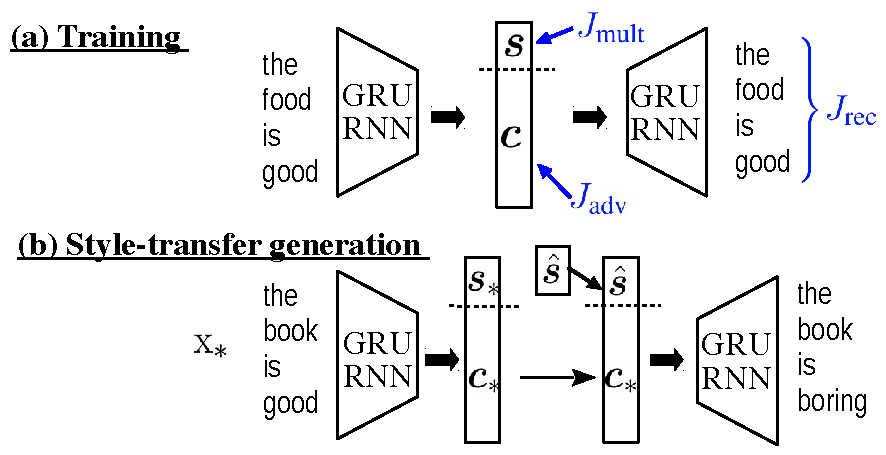
\includegraphics[width=0.9\linewidth]{model-overview}
	\caption{Model Overview}
	\label{fig:model-overview}
\end{figure*}

\section{Introduction}

The neural network has been a successful learning machine during the past decade due to its high modeling capability, which arises from multiple layers of non-linear transformation of input features. Such transformations, however, make intermediate features `latent', in that they do not have explicit meaning and are not explainable. Therefore, neural networks are usually treated as black-box machinery.

Disentangling the latent space of neural networks has become an increasingly important research topic. In the image domain, for example, \newcite{chen2016infogan} use adversarial and information maximization objectives to produce interpretable latent representations that can be tweaked to adjust writing style for handwritten digits, as well as lighting and orientation for face models. \newcite{mathieu2016disentangling} utilize a convolutional autoencoder to achieve the same objective. However, this problem is not well explored in natural language processing (NLP).

In this paper, we address the problem of disentangling neural networks' latent space for text generation. Our model is built on an autoencoder that learns the latent space (vector representation) of a sentence by decoding the sentence itself. We would like the latent space to be disentangled with different features, namely, \textit{style} and \textit{content}.

To accomplish this, we propose a simple approach that combines multi-task loss and adversarial loss. We artificially divide the latent representation into two parts: style space and content space.
We learn model parameters that produce separate style and content latent spaces from the encoded sentence representation. The multi-task objective operates on the style space to ensure it does contain style information.
The adversarial objective, on the contrary, operates on the content space to minimize the predictability of style. In this way, the style and content parts can be disentangled from each other.

The disentangled latent space can be directly used for style transfer in sentence generation~\cite{fu2017style,shen2017style}, where a system can generate a sentence with the same content, but a different style. We simply apply an autoencoder to encode the content vector of a sentence, but ignore its encoded style vector. Then we infer from the training data, an empirical embedding of the style that we want to transfer. The encoded content vector and the inferred style vector are concatenated and fed to the autoencoder for decoding. Using this grafting technique, we generate a new sentence similar in meaning but different in sentiment.

We conducted experiments on a product review benchmark dataset. Both qualitative and quantitative results show that the style vector does contain most style information, whereas the content vector contains little (if any). In the style-transfer experiment, we achieve significantly better style transfer scores than previous results, while obtaining better or comparable content preservation scores.  We also show in an ablation test, that the two auxiliary losses can be combined well, each playing its own role in disentangling latent space.


\section{Related Work}


Disentangling latent space has been widely explored in the image processing domain, where researchers have successfully disentangled rotation features, color features, etc.~\cite{chen2016infogan,luan2017deep}. Some image styles (e.g. artistic style) can be well captured by certain statistics~\cite{gatys2016image}. For other styles, researchers adopt various data augmentation techniques to train a disentangled latent space~\cite{champandard2016semantic,kulkarni2015deep}.

In natural language processing, the `style' itself is vague, and as a convenient starting point, NLP researchers typically treat sentiment as a salient style of text. \newcite{hu2017toward} manage to control the sentiment by reconstructing sentiment and content based on generated sentences. However, there is no evidence that the latent space could be disentangled by such reconstruction. \newcite{fu2017style} propose two approaches, using style embedding or two specifically trained decoders for style transfer. They apply the adversarial loss on the encoded space to discourage style encoding. \newcite{shen2017style} use an adversarial discriminator to align the recurrent hidden decoder states of (a) sentences with a given style and (b) sentences to be transferred to the given style, thereby performing style transfer.

Our paper differs from the previous work in that both our style space and content space are encoded from the input. We apply two auxiliary losses to ensure that each space encodes its own information. Our disentangled space can be directly applied to style-transfer sentence generation, as in the aforementioned studies.


\begin{figure}[ht]
	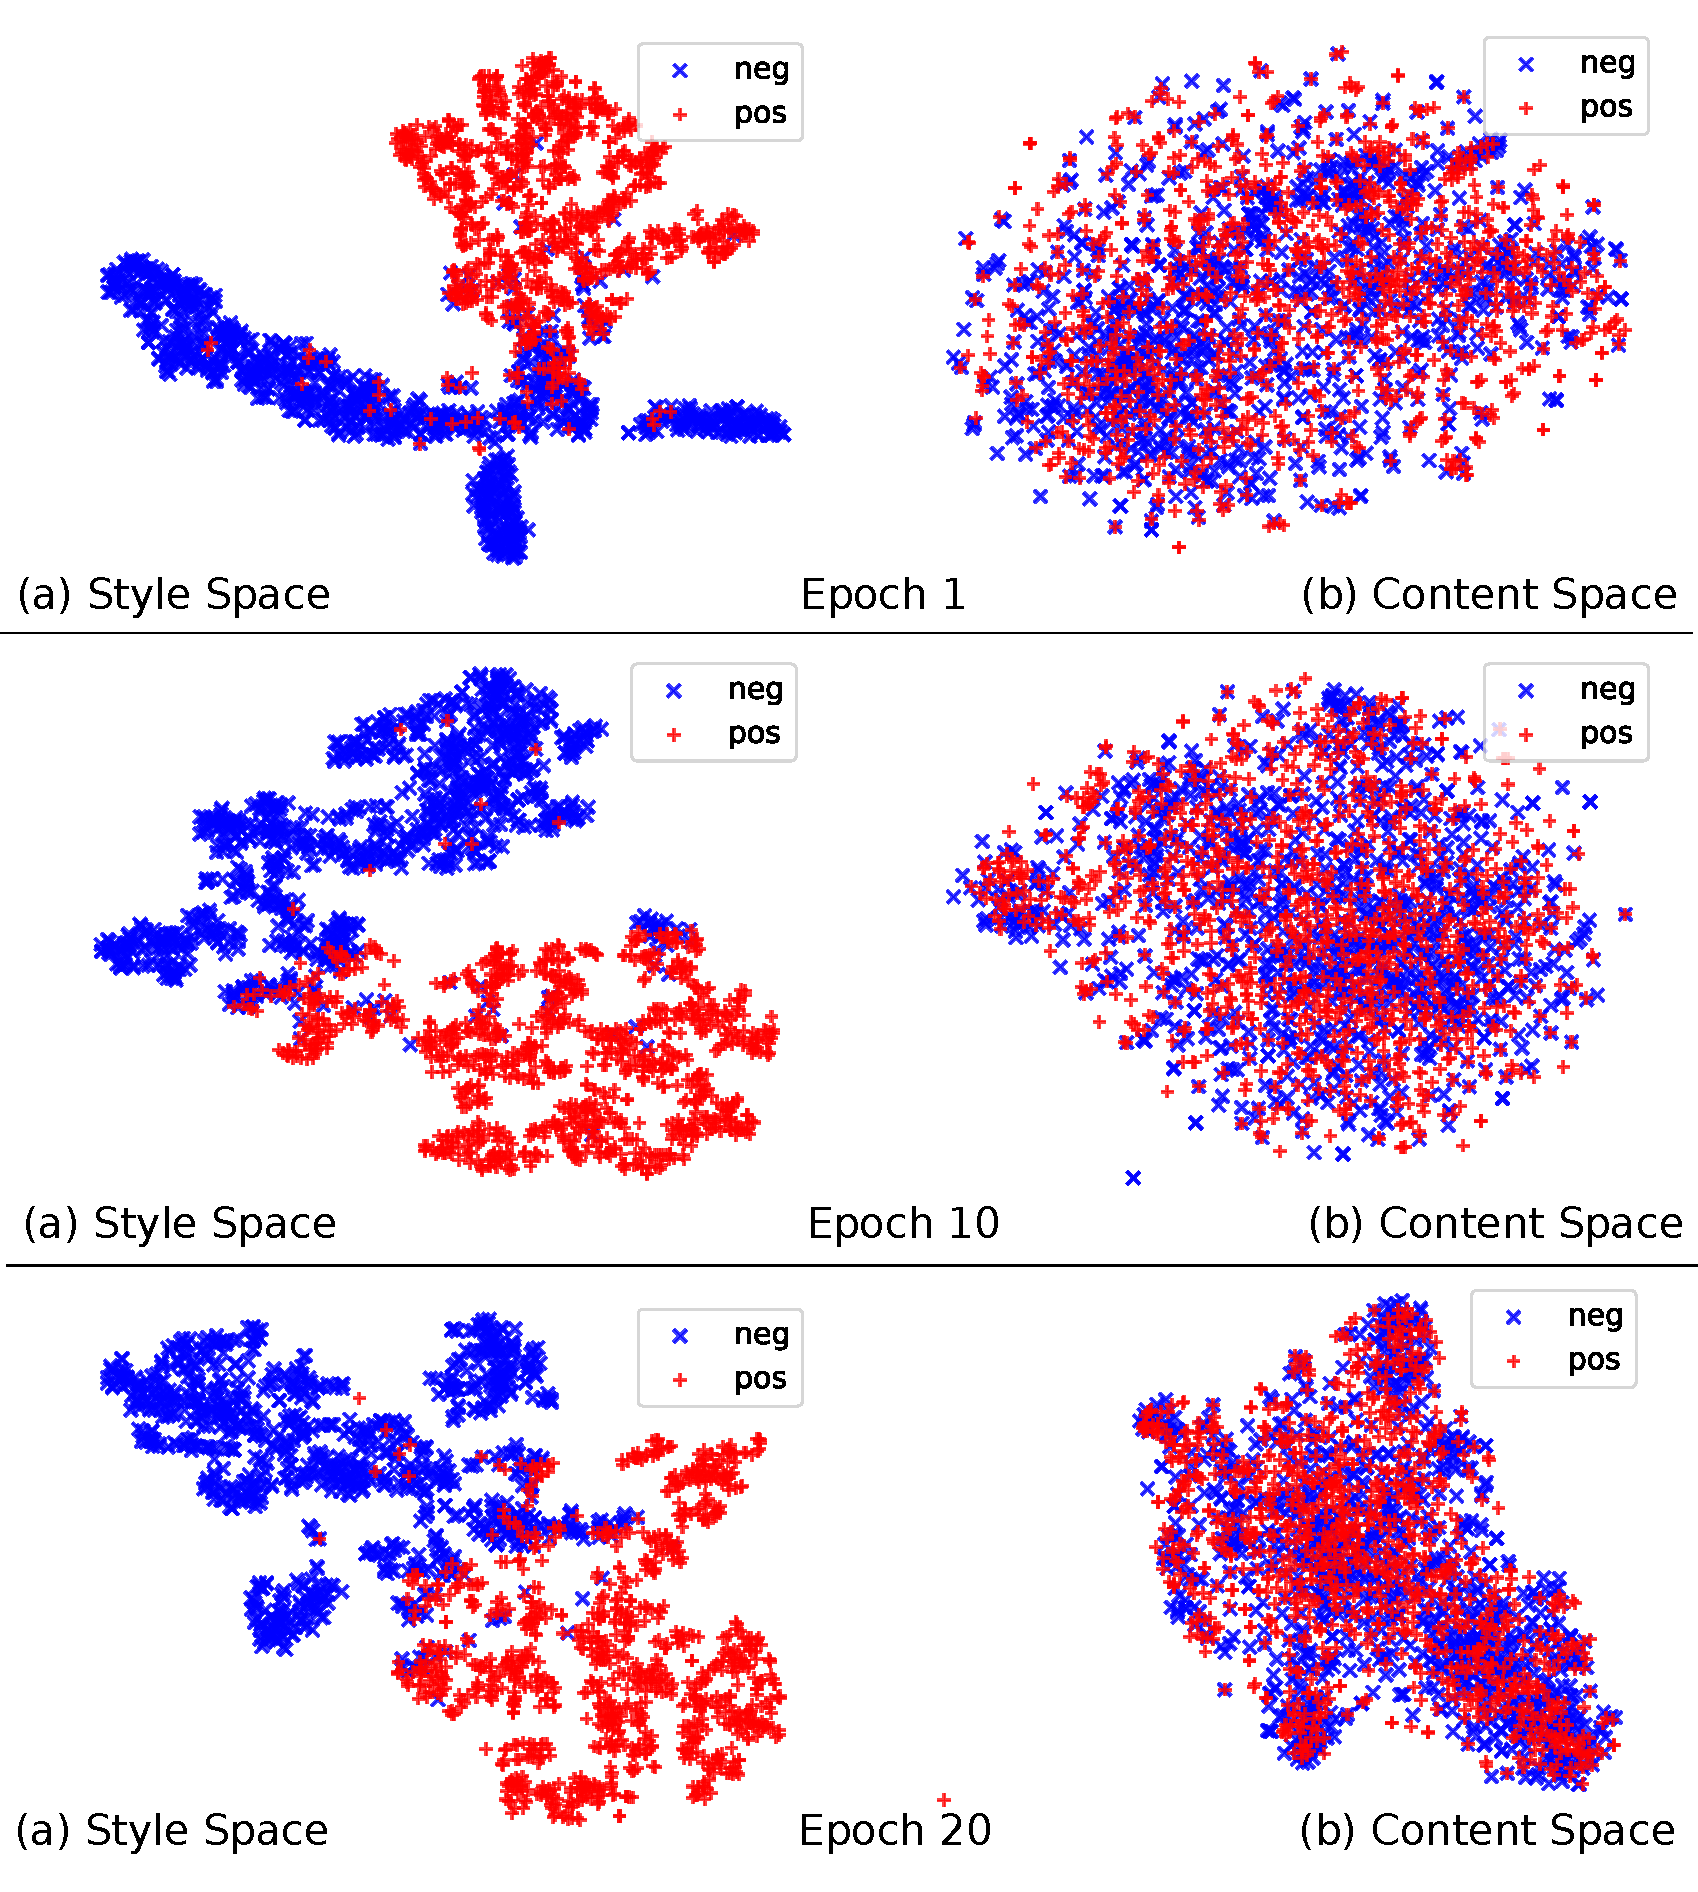
\includegraphics[width=\linewidth]{latent-spaces-dae}
	\caption{T-SNE Plots: (a) Style and (b) Content Spaces - DAE Model}
	\label{fig:dae-tsne}
\end{figure}

\begin{figure}[ht]
	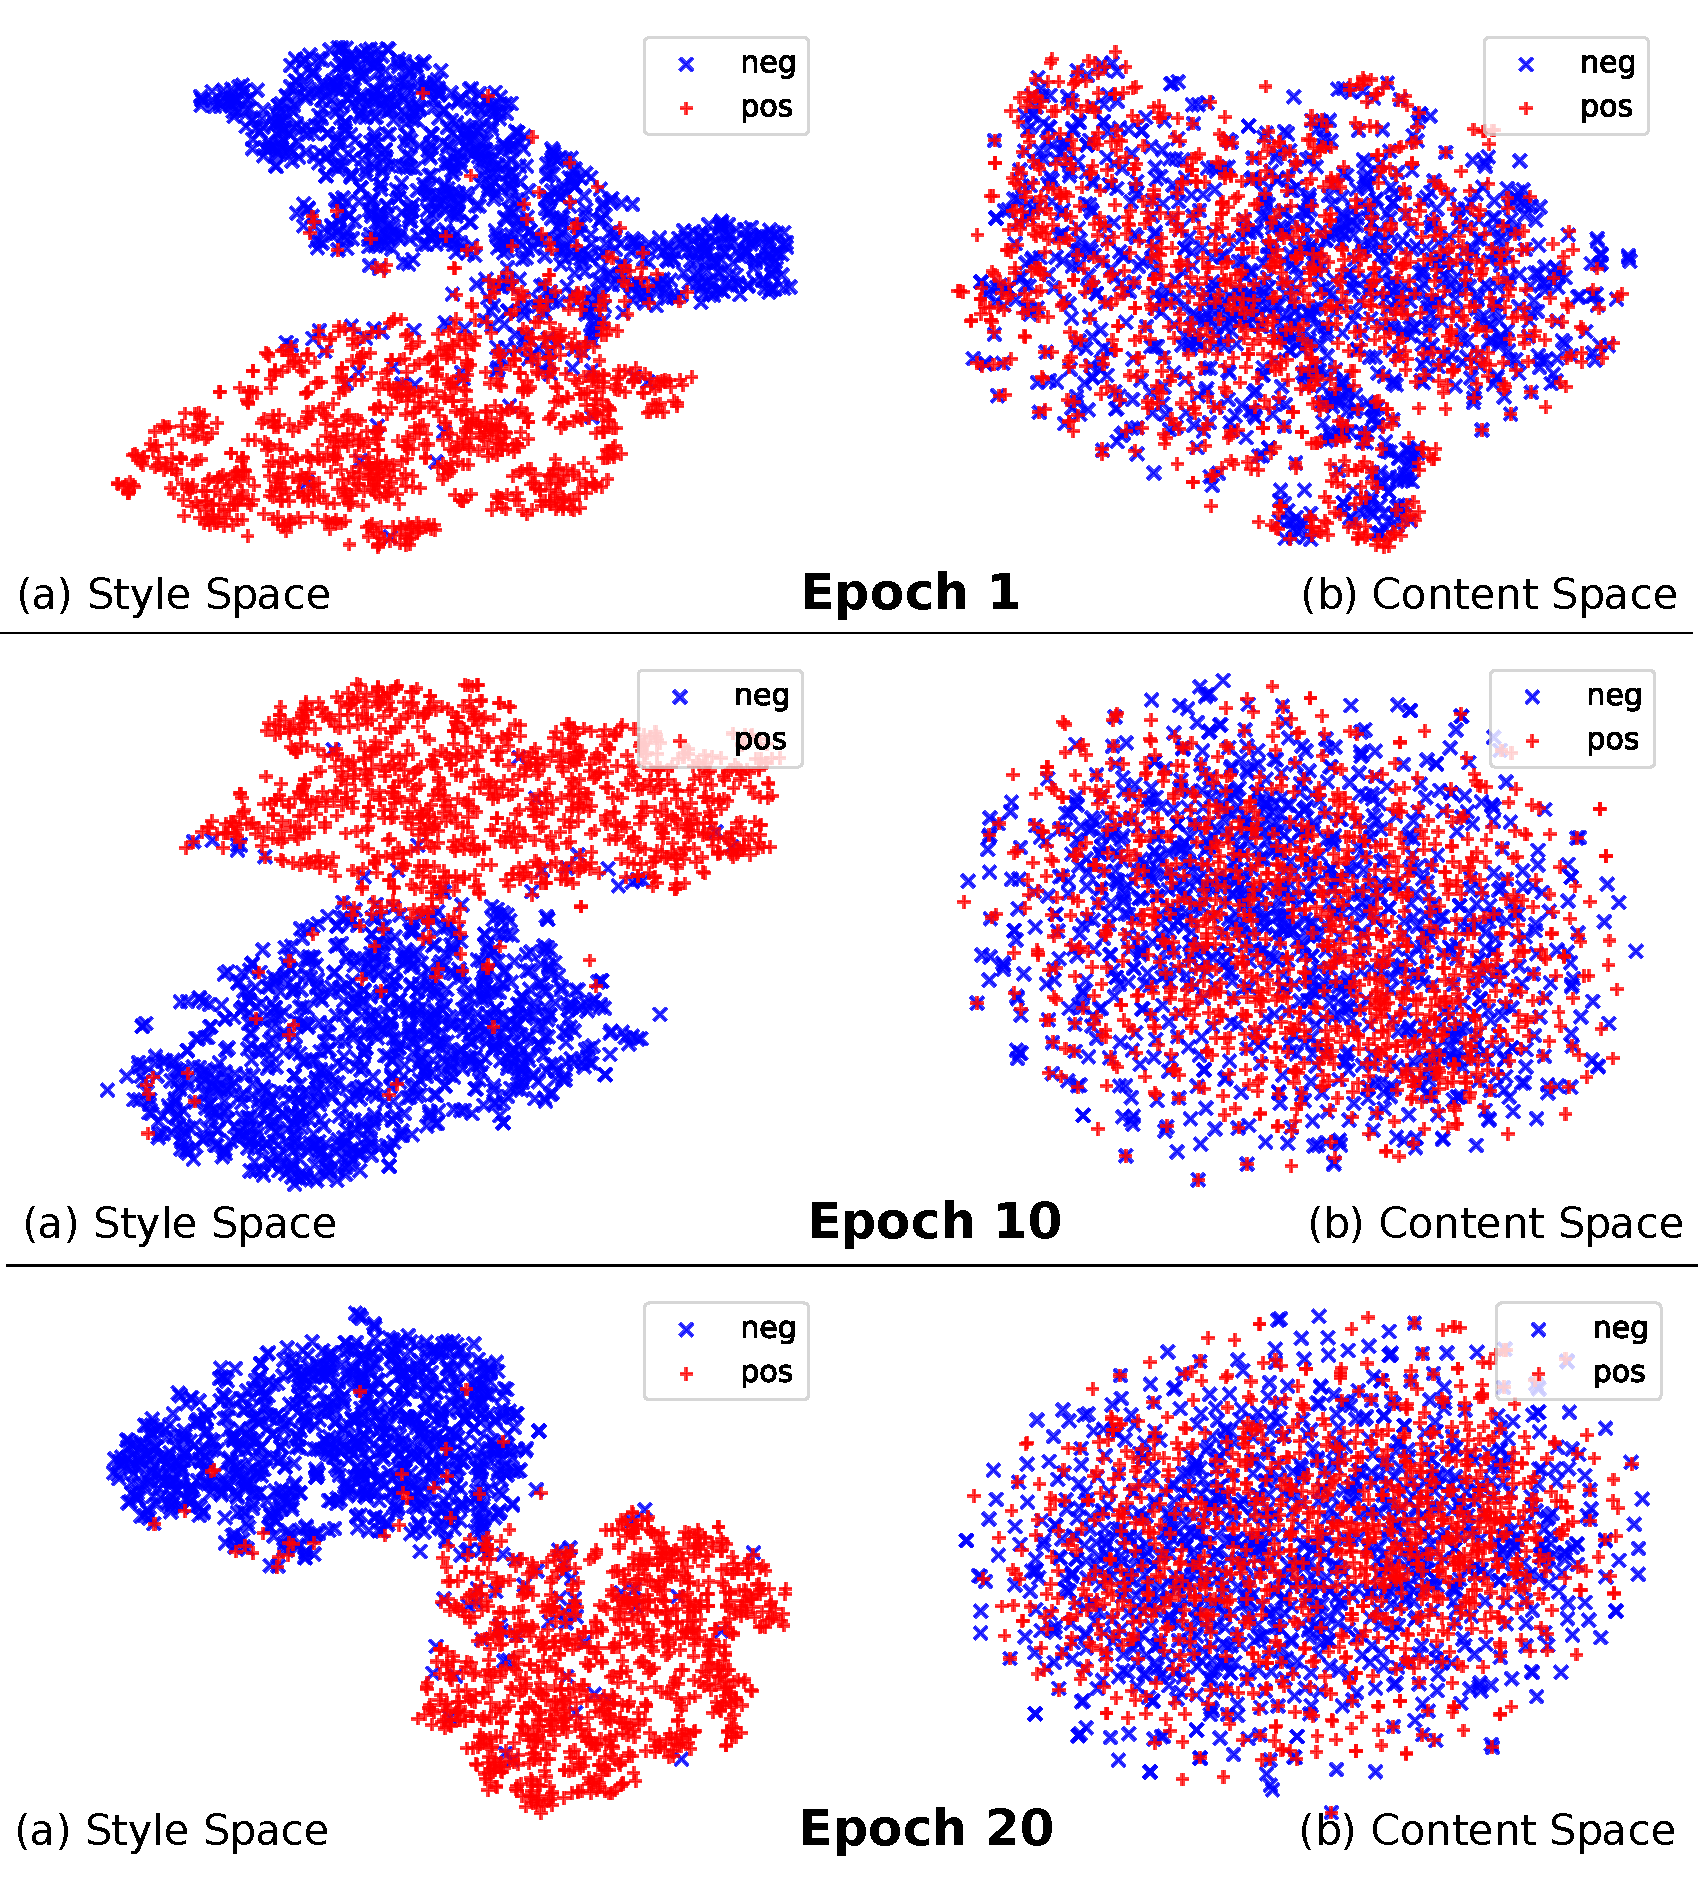
\includegraphics[width=\linewidth]{latent-spaces-vae}
	\caption{T-SNE Plots: (a) Style and (b) Content Spaces - VAE Model}
	\label{fig:vae-tsne}
\end{figure}


\section{Approach}

In this section, we describe our approach in detail. Our model is built upon an autoencoder with a sequence-to-sequence (Seq2Seq) neural network~\cite{sutskever2014sequence}, as described in Subsection~\ref{ss:seq2seq}. Then we introduce two auxiliary losses, multi-task loss and adversarial loss in Subsections~\ref{ss:multi} and \ref{ss:adv}, respectively. Subsection~\ref{ss:prediction} presents the approach to transfer style in natural language generation. Figure~\ref{fig:model-overview} depicts both training and prediction processes of our approach.


\subsection{Autoencoder} \label{ss:seq2seq}

An autoencoder encodes an input to a latent vector space, from which it decodes the input itself. By doing so, the autoencoder learns meaningful representations of data. This serves as our primary learning objective. Besides, we also use the autoencoder for text generation in the style-transfer application.

Let $\rmx=(x_1, x_2, \cdots x_n)$ be an input sentence. The encoder encodes $\rm x$ by a recurrent neural network (RNN) with gated recurrent units (GRU) \cite{cho2014learning}, and obtains a hidden state $\bm h$.

Then a decoder RNN generates a sentence, which ideally should be $\rmx$ itself. Suppose at a time step $t$, the decoder RNN predicts the word $x_t$ with probability $p(x_t|\bm h, x_1\cdots x_{t-1})$, then the autoencoder is trained with cross-entropy loss, given by
\begin{equation}\nonumber
	\loss{rec}(\bm\theta_E,\bm\theta_D)= -\sum_{t=1}^n \log
	p(x_t|\bm h, x_1\cdots x_{t-1})
\end{equation}
where $\bm\theta_E$ and $\bm\theta_D$ are the parameters of the encoder and decoder, respectively.

Since this loss trains the autoencoder to reconstruct $\rmx$, it is also called \textit{reconstruction loss}.

Besides the above reconstruction loss, we design two auxiliary losses to disentangle the latent space $\bm h$. In particular, we hope that $\bm h$ can be separated into two spaces $\bm s$ and $\bm c$, representing style and content respectively, i.e., $\bm h = [\bm s ; \bm c]$, where $[\cdot;\cdot]$ denotes concatenation. This is accomplished by the below auxiliary losses.

\begin{table*}[ht]
	\centering
	\begin{tabular}{| l | r | r |}
		\hline
		                                        & \tabh{DAE}                  & \tabh{VAE} \\
		\hline \hline
		Random/Majority guess                   & \multicolumn{2}{c|}{0.6018}              \\ \hline \hline
		Content latent space  ($\bm c$)         & 0.6137                      & 0.6567     \\ \hline
		Style latent space ($\bm s$)            & 0.7927                      & 0.7911     \\ \hline
		Complete latent space ($[\bm s;\bm c]$) & 0.7918                      & 0.7918     \\
		\hline
	\end{tabular}
	\caption{Style classification accuracy.}
	\label{tab:classification}
\end{table*}


\subsection{Multi-Task Loss} \label{ss:multi}

Our first auxiliary loss ensures the style space does contain style information. We build a classifier on the style space $\bm s$ predicting the style label $s$, which is a part of the training data.

This loss can be viewed as a \textit{multi-task} loss, which makes the neural network not only decode the sentence, but also predicts its sentiment. Similar multi-task losses are used in previous work for sequence-to-sequence learning \cite{luong2015multi}, sentence representation learning \cite{jernite2017discourse} and sentiment analysis \cite{balikas2017multitask}, among others.

In our application, we follow previous work \cite{hu2017toward,shen2017style,fu2017style} and treat the sentiment as the style of interest. We introduce a multi-label classifier
\begin{equation}
	p(s=1|\bm s;\bm\theta_\text{mult})=\sigma(\bm w_\text{mult}^\top \bm s + b_\text{mult})
\end{equation}
where $\bm\theta_\text{mult}=[\bm w_\text{mult}; b_\text{mult}]$ are the classifier's parameters for multi-task learning.
\begin{align} \label{eqn:Jmult}
	 & \loss{mult}(\bm\theta_{E};\bm\theta_\text{mult})=                  \\ \nonumber
	 & -s\log p_\text{mult}(s|\bm s) - (1-s)\log p_\text{mult}(1-s|\bm s)
\end{align}
where $\bm\theta_E$ are the encoder's parameters. (Notice that the bold letter $\bm s$ represents the encoded style vector, whereas the unbold letter $s$ represents the binary style label).


\subsection{Adversarial Learning} \label{ss:adv}

The above multi-task loss only operates on the style space, but does not have an effect on the content space $\bm c$.

We therefore apply an adversarial loss to disentangle the content space from style information, inspired by adversarial generation~\cite{goodfellow2014generative}, adversarial domain adaptation~\cite{liu2017adversarial}, and adversarial style transfer~\cite{fu2017style}.

The idea of adversarial loss is to introduce an adversary that deliberately discriminates style $s$ on the content vector $\bm c$. Then the autoencoder is trained to learn such a content vector space that its adversary cannot predict style information.

Concretely, the adversarial discriminator predicts style $s$ by a logistic regression
\begin{equation}
	p_\text{dis}(s=1|\bm c;\bm\theta_\text{adv})=\sigma(\bm w_\text{adv}^\top \bm c + b_\text{adv})
\end{equation}
where $\bm\theta_\text{dis}=[\bm w_\text{dis}; b_\text{dis}]$ are the parameters of the adversary. It is trained by
\begin{align}
	 & \loss{dis}(\bm\theta_\text{dis})=                              \\ \nonumber
	 & -s\log p_\text{dis}(s|\bm c)-(1-s)\log p_\text{dis}(1-s|\bm c)
\end{align}
The adversarial loss appears similar to the multi-task loss as in Eq.~(\ref{eqn:Jmult}). However, it should be emphasized that, for the adversary, the gradient is not propagated back to the autoencoder, i.e., $\bm c$ is treated as shallow features.

Having trained an adversary, we would like the autoencoder to be tuned in such an \textit{ad hoc} fashion, that $\bm c$ is not discriminative in style. In other words, we penalize the entropy of the adversary's prediction, given by
\begin{equation}
	\loss{adv}(\bm\theta_E)=\mathcal{H}(p_\text{dis}(s|\bm c))
\end{equation}
where $\mathcal{H}=-\sum_{i\in\text{labels}}p_i\log p_i$ is the entropy. The adversarial objective is maximized, in this phase, with respect to the encoder.

\todo[inline]{Add note about BoW adversarial objective}


\subsection{Training Process}

To put it all together, our training process is a loop of the following processes:
\begin{itemize}
	\item minimize $\loss{dis}(\bm\theta_\text{dis})$ w.r.t. $\bm\theta_\text{dis}$, and
	\item minimize $\loss{rec}(\bm\theta_E, \bm\theta_D) + \lambda_\text{mult}(\bm\theta_E,\bm\theta_\text{mult}) -\lambda_\text{adv}
		      \loss{adv}(\theta_E)$ w.r.t. $\bm\theta_E, \bm\theta_D, \bm\theta_\text{mult}$.
\end{itemize}
where $\lambda_\text{mult}$ and $\lambda_\text{adv}$ balance these losses.

We use the Adam optimizer \cite{kingma2014adam} with an initial learning rate of $10^{-3}$ and train the model for 20 epochs. Both the autoencoder and its adversary are trained once per epoch with $\lambda_\text{mult} = 1$ and $\lambda_\text{adv} = 0.3$.

\subsection{Generating Style-Transferred Sentences} \label{ss:prediction}

A direct application of our disentangled latent space is style transfer for natural language generation. For example, we can generate a sentence with generally the same meaning (content) but an opposite sentiment.

Let $\rmx_*$ be an input sentence with $\bm s_*$ and $\bm c_*$ being the encoded, disentangled style and content vectors, respectively. If we would like to transfer its content to a different style, we compute an empirical estimate of the target style's vector $\hat{\bm s}$ by
\begin{equation*}
	\hat{\bm s}=\frac{\sum_{i\in\text{target style}}\bm s_i}{\text{\# target style samples}}
\end{equation*}
The inferred target style $\hat{\bm s}$ is concatenated with the encoded content $\bm c_*$ for decoding (Figure~\ref{fig:model-overview}b).


\begin{table*}[ht]
	\centering
	\begin{tabular}{| l | r | r | r | r |}
		\hline
		\tabc{2}{Model}                       & \tabh{Transfer} & \tabh{Content}      & \tabh{Word}    & \tabh{Language} \\
		                                      & \tabh{Strength} & \tabh{Preservation} & \tabh{Overlap} & \tabh{Fluency}  \\
		\hline
		\hline
		Cross-Alignment \citep{shen2017style} & 0.8087          & 0.8920              & 0.2087         & 23.3886         \\
		\hline
		Style Embedding \citep{fu2017style}   & 0.1819          & 0.9586              & 0.6661         & 16.1711         \\
		\hline
		Ours (DAE)                            & 0.8425          & 0.8924              & 0.2552         & 16.4808         \\
		\hline
		Ours (VAE)                            & 0.8903          & 0.8824              & 0.2105         & 14.4099         \\
		\hline
	\end{tabular}
	\caption{Yelp Dataset - Comparison with previous approaches.}
	\label{tab:yelp-comparison-previous}
\end{table*}

\begin{table*}[ht]
	\centering
	\begin{tabular}{| l | r | r | r | r |}
		\hline
		\tabc{2}{Model}                       & \tabh{Transfer} & \tabh{Content}      & \tabh{Word}    & \tabh{Language} \\
		                                      & \tabh{Strength} & \tabh{Preservation} & \tabh{Overlap} & \tabh{Fluency}  \\
		\hline
		\hline
		Cross-Alignment \citep{shen2017style} & 0.6063          & 0.8933              & 0.0241         & 26.3093         \\
		\hline
		Style Embedding \citep{fu2017style}   & 0.4165          & 0.9332              & 0.3588         & 28.1346         \\
		\hline
		Ours (DAE)                            & 0.7032          & 0.9178              & 0.1305         & 32.4184         \\
		\hline
		Ours (VAE)                            & 0.7259          & 0.9090              & 0.0814         & 28.4953         \\
		\hline
	\end{tabular}
	\caption{Amazon Dataset - Comparison with previous approaches.}
	\label{tab:amazon-comparison-previous}
\end{table*}



\begin{table*}[ht]
	\centering
	\begin{tabular}{| l | r | r | r | r |}
		\hline
		\tabc{2}{Objectives}                                     & \textbf{Transfer} & \textbf{Content}      & \textbf{Word}    & \textbf{Language} \\
		                                                         & \textbf{Strength} & \textbf{Preservation} & \textbf{Overlap} & \textbf{Fluency}  \\
		\hline
		\hline
		$\loss{rec}$                                             & 0.1436            & \textbf{0.9154}       & \textbf{0.3288}  & 14.2781           \\
		\hline
		$\loss{rec}$, $\loss{adv}$                               & 0.7274            & 0.8800                & 0.2037           & 14.1567           \\
		\hline
		$\loss{rec}$, $\loss{mult}$                              & 0.7894            & 0.8976                & 0.2589           & 14.5607           \\
		\hline
		$\loss{rec}$, $\loss{badv}$                              & 0.1677            & 0.9147                & 0.3282           & 14.4486           \\
		\hline
		$\loss{rec}$, $\loss{adv}$, $\loss{mult}$                & \textbf{0.8903}   & 0.8824                & 0.2105           & 14.4099           \\
		\hline
		$\loss{rec}$, $\loss{adv}$, $\loss{badv}$                & 0.7491            & 0.8827                & 0.2022           & 14.3568           \\
		\hline
		$\loss{rec}$, $\loss{mult}$, $\loss{badv}$               & 0.7832            & 0.8958                & 0.2567           & 14.3373           \\
		\hline
		$\loss{rec}$, $\loss{adv}$, $\loss{mult}$, $\loss{badv}$ & 0.8846            & 0.8782                & 0.1970           & \textbf{14.0479}  \\
		\hline
	\end{tabular}
	\caption{Ablation test.}
	\label{tab:ablation-results}
\end{table*}

\section{Experiments}

We conduct experiments on two datasets, the details for which are given below.

\subsection{Yelp Service Reviews}

We use a subset of the Yelp review dataset \citep{challenge2013yelp}, which has been sourced from the code repository accompanying the implementation of the paper by \cite{shen2017style} open-sourced by the authors~\footnote{\url{https://github.com/shentianxiao/language-style-transfer}}. It contains 444101, 126670 and 63483 sentences for train, validation, and test, respectively, each sampling accompanied by binary sentiment labels. The maximum sentence length is 15, and the vocabulary size is about 9200.

\subsection{Amazon Product Reviews}

We also use an Amazon product reviews dataset~\footnote{\url{http://jmcauley.ucsd.edu/data/amazon/}}, following \cite{fu2017style}. The reviews were sourced from the code repository accompanying the paper~\footnote{\url{https://github.com/fuzhenxin/text_style_transfer}}. It contains 559142, 2000, 2000 sentences for train, validation, and test, respectively, each sampling accompanied by binary sentiment labels. The maximum sentence length is 20, and the vocabulary size is about 58000.

\subsection{Disentangling Latent Space}


We first analyze how the style (sentiment) and content of the latent space are disentangled. We train a logistic classifier based on different latent spaces, and show results in Table~\ref{tab:classification}.

We see that the 128-dimensional content vector $\bm c$ is not discriminative for style. It achieves an accuracies that are only slightly better than random/majority guess. However, the 8-dimensional style vector $\bm s$, despite its low dimensionality, achieves significantly higher style classification accuracy. When combining content and style vectors, we achieve no further improvement. These results verify the effectiveness of our disentangling approach, because the style space does contain style information, whereas the content space doesn't.

We show t-SNE plots of both the deterministic autoencoder (DAE) and the variational autoencoder (VAE) models in Figure \ref{fig:dae-tsne} and Figure \ref{fig:vae-tsne}, respectively.


As can be seen from the t-SNE plots, sentences with different styles are noticeably separated in a cleaner manner in the style space (LHS), but are indistinguishable in the content space (RHS). It is also evident that the latent space learned by the variational autoencoder is significantly smoother and continuous than the one learned by the deterministic autoencoder.


\subsection{Style-Transfer Sentence Generation}

We apply the disentangled latent space to a style-transfer sentence generation task, where the goal is to generate a sentence with different sentiment (style). We followed~\newcite{fu2017style} and used two metrics: (1) For style transfer, we train a style classifier and predict the accuracy of the generated sentences. While the style classifier itself may not be perfect, it provides a quantitative way of evaluating the strength of style transfer. (2) For the content-preservation score, we compute a sentence embedding by min, max, and average pooling of word embeddings; then a cosine similarity is computed to evaluate how close two sentences are in meaning. Here, sentiment words from a stop list \cite{hu2004mining} are removed.

We compare our approach with state-of-the-art previous work in Table~\ref{tab:yelp-comparison-previous}. We re-conducted the experiments with their publicly available code on our data splits.
Results show that, our approach achieves a comparable content-preservation score with previous work, but a significantly better style-transfer score, showing that our disentangled latent space can be used for better style-transfer sentence generation.

Table~\ref{tab:ablation-results} presents the results of an ablation test. We see that both adversarial loss and reconstruction loss play a role in the strength of style transfer, and that they can be combined to further improve performance.


Some examples of style-transfer sentence generation are illustrated in Table~\ref{tab:transfer-samples}. We see that, with the empirically estimated style vector, we can flexibly control the sentiment of generated sentences.


\begin{table*}[ht]
	\centering
	\begin{tabular}{| p{0.3\linewidth} | p{0.3\linewidth} | p{0.3\linewidth} |}
		\hline
		\tabc{2}{Original (Positive)}                          & \tabh{DAE Transferred}                                         & \tabh{VAE Transferred}                                      \\
		                                                       & \tabh{(Negative)}                                              & \tabh{(Negative)}                                           \\
		\hline
		i would recommend a visit here                         & i would not recommend this place again                         & i would not recommend this place for my experience          \\
		\hline
		the restaurant itself is romantic and quiet            & the restaurant itself is soooo quiet                           & the restaurant itself was dirty                             \\
		\hline
		my experience was brief but very good                  & my experience was very loud and very expensive                 & my experience was ok but not very much                      \\
		\hline
		the food is excellent and the service is exceptional   & the food is by the worst part is the horrible costumer service & the food was bland and i am not thrilled with this          \\
		\hline
		the food is very very amazing like beef and fish       & the food is very horrible i have ever had mostly fish          & the food is very bland and just not fresh                   \\
		\hline
		we will definitely come back here                      & we will not come back here again                               & we will never come back here                                \\
		\hline
		both were very good                                    & everything was very bland                                      & both were very bad                                          \\
		\hline
		\hline
		\tabc{2}{Original (Negative)}                          & \tabh{DAE Transferred}                                         & \tabh{VAE Transferred}                                      \\
		                                                       & \tabh{(Positive)}                                              & \tabh{(Positive)}                                           \\
		\hline
		\hline
		so nasty                                               & so helpful                                                     & so fabulous                                                 \\
		\hline
		consistently slow                                      & consistently awesome                                           & fast service                                                \\
		\hline
		crap fries hard hamburger buns burger tasted like crap & cheap and yummy sandwiches really something different          & yummy hamburgers and blue cheese bagels are classic italian \\
		\hline
		oh and terrible tea                                    & oh and awesome tea                                             & oh and great tea                                            \\
		\hline
		the interior is old and generally falling apart        & the interior is clean and orderly as entertaining              & the interior is old and noble                               \\
		\hline
		front office customer service does not exist here      & front office is very professional does you                     & kudos to customer service is very professional              \\
		\hline
		the crust was kinda gooey like                         & the crust is kinda traditional                                 & the crust is soooooo worth it                               \\
		\hline
	\end{tabular}
	\caption{Examples of style-transfer generation.}
	\label{tab:transfer-samples}
\end{table*}

\section{Conclusion and Future Work}
In this paper, we propose a simple yet effective approach for disentangling the latent space of neural networks by multi-task loss and adversarial loss. Our disentangled space can be applied to style-transfer sentence generation, achieving similar content-preservation score but significantly higher style-transfer strength compared to previous state-of-the-art work.

In future work, we would like to disentangle the latent space of variational autoencoders (VAEs), as VAE provides a more robust way of generating sentences from a continuous space~\cite{bowman2016generating}. In VAE, the adversarial loss could be applied to posterior distributions, as opposed to an encoded content vector in our paper.

\bibliography{emnlp2018}
\bibliographystyle{acl-natbib}

\end{document}
